\documentclass[10pt,letterpaper]{article}
\usepackage[margin=0.75in]{geometry}
\usepackage{amsmath,amssymb,bm,graphicx,booktabs}
\usepackage[colorlinks=true,allcolors=blue]{hyperref}
\usepackage{fancyhdr}
\pagestyle{fancy}\fancyhf{}\fancyhead[L]{Supplemental Material --- Draft v6}\fancyhead[R]{October 13, 2026}\fancyfoot[C]{\thepage}
\setlength{\headheight}{13pt}
\setlength{\parindent}{1em}\setlength{\parskip}{3pt}
\renewcommand{\theequation}{S\arabic{equation}}
\renewcommand{\thetable}{S\arabic{table}}
\renewcommand{\thefigure}{S\arabic{figure}}
\newcommand{\F}{\mathcal F}\newcommand{\B}{\mathcal B}
\newcommand{\fld}[1]{\mathsf{#1}}
\newcommand{\norm}[1]{\left\lVert#1\right\rVert}
\begin{document}
\begin{center}
{\large\bfseries Supplemental Material for\\[3pt] Residual Carleman lift for nonlinear lattice Boltzmann simulations}
\end{center}
\section*{S1. Population update and six-field implementation}
We use conventional LB component notation. The connection to the global field in the main text is
\begin{equation}
 [\fld f_n]_{i,\bm x}=f_i(\bm x,n),\qquad
 \fld f_n\in\mathbb R^{9N^2},\qquad f_i^{(0)}(\bm x)=\rho_0w_i.
\end{equation}
The index $n$ denotes time, $i$ labels a discrete velocity $\bm v_i\in\{-1,0,1\}^2$, and $\bm x$ labels a node. Bold symbols denote physical spatial vectors. D2Q9 weights are $w_i=w(v_{ix})w(v_{iy})$, with $w(0)=2/3$, $w(\pm1)=1/6$, and $c_s^2=1/3$. Populations are sampled immediately after collision. In lattice units the streamed populations and moments are
\begin{equation}
 f_i^s(\bm x,n)=f_i(\bm x-\bm v_i,n),\qquad
 \rho=\sum_i f_i^s,\quad \bm j=\sum_i\bm v_i f_i^s,\quad \bm u=\bm j/\rho.
 \label{eq:stream}
\end{equation}
Unless displayed, moment arguments are $(\bm x,n)$. The equilibrium and stress projection are
\begin{align}
 f_i^{\rm eq}(\rho,\bm j)&=w_i\left[\rho+\frac{\bm v_i\cdot\bm j}{c_s^2}
 +\frac{H_{i\alpha\beta}j_\alpha j_\beta}{2c_s^4\rho}\right],
 &H_{i\alpha\beta}&=v_{i\alpha}v_{i\beta}-c_s^2\delta_{\alpha\beta},\label{eq:feq}\\
 (\mathcal R_2h)_i&=\frac{w_i}{2c_s^4}H_{i\alpha\beta}\sum_jH_{j\alpha\beta}h_j.
 \label{eq:R2}
\end{align}
Repeated Cartesian indices are summed. The complete regularized update is
\begin{equation}
 f_i(\bm x,n+1)=f_i^{\rm eq}(\rho,\bm j)
 +(1-\omega)\big[\mathcal R_2(f^s-f^{\rm eq})\big]_i(\bm x,n),\qquad \omega=1/\tau.
 \label{eq:model}
\end{equation}
Thus $\F=\mathcal C\mathcal S$ is a full stream--collide map, not a collision increment. Uniform rest, $f_i^{(0)}=\rho_0w_i$, is left unchanged by both operations. Expanding Eq.~\eqref{eq:feq} at $(\rho_0,\bm0)$ gives the conventional quadratic equilibrium
\begin{equation}
 f_i^{\rm eq}=\rho_0w_i+w_i\left[\delta\rho+\frac{\bm v_i\cdot\bm j}{c_s^2}
 +\frac{H_{i\alpha\beta}j_\alpha j_\beta}{2c_s^4\rho_0}\right]
 +O(\delta\rho\,|\bm j|^2).
 \label{eq:restexpansion}
\end{equation}
The remainder starts at degree three in $(\delta\rho,\bm j)$; retaining $1/\rho$ instead gives the rational equilibrium actually used by the direct LB reference.

The postcollision state lies exactly in the six-dimensional local Hermite subspace. Put $h_0(v)=1$, $h_1(v)=\sqrt3v$, $h_2(v)=(3v^2-1)/\sqrt2$, and let $\mathcal J=\{(0,0),(1,0),(0,1),(2,0),(1,1),(0,2)\}$. Then
\begin{equation}
 a_{pq}(\bm x,n)=\sum_i h_p(v_{ix})h_q(v_{iy})f_i(\bm x,n),\qquad
 f_i(\bm x,n)=w_i\sum_{(p,q)\in\mathcal J}h_p(v_{ix})h_q(v_{iy})a_{pq}(\bm x,n).
 \label{eq:moments}
\end{equation}
The local array is $\fld a=(\rho,\sqrt3j_x,\sqrt3j_y,a_{20},a_{11},a_{02})$. Streaming followed by extraction defines a linear six-field map $T$. If its output has conserved coordinates $(\rho,p_x,p_y)$, collision keeps them and updates its stress coordinates as
\begin{equation}
 (a_{20},a_{11},a_{02})'=(1-\omega)(a_{20},a_{11},a_{02})
 +\frac{\omega}{\rho}\left(\frac{p_x^2}{\sqrt2},p_xp_y,\frac{p_y^2}{\sqrt2}\right),\qquad (p_x,p_y)=\sqrt3\bm j.
 \label{eq:collision6}
\end{equation}
Equations~\eqref{eq:moments}--\eqref{eq:collision6} specify the implementation; they introduce no further model approximation. Applied at all sites, the moment extraction $\mathcal H$ and reconstruction $\mathcal R$ map between the global postcollision subspace and $\mathbb R^{6N^2}$. Operators and pair tensors transform accordingly: $\widehat A=\mathcal H A\mathcal R$, $\widehat\B=\mathcal H\B(\mathcal R\otimes\mathcal R)$, and $\widehat Z=(\mathcal H\otimes\mathcal H)\fld Z$.

\newpage
\section*{S2. Background preparation and population residual}
Specify the flow, Reynolds number, horizon $0\leq t^*\leq T^*$, and ordered pair $(N_c,N_t)$ before preparation. The purpose is to supply nonlinear background dynamics that make a truncated residual lift accurate over this entire interval. The coarse populations $f_i^c(\bm x_c,m)=[\fld g_m]_{i,\bm x_c}$ evolve by Eq.~\eqref{eq:model} on $N_c^2$ sites with $\tau_{N_c}$; the target LB map $\F_t$ uses $N_t^2$ sites and $\tau_{N_t}$. With the same lattice velocity $U$, $t^*=Um/N_c=Un/N_t$ at corresponding times. The step counts are $M_c=T^*N_c/U$ and $M_t=T^*N_t/U$ (integers in our tests).

Let $\mathcal P_{c\to t}$ denote Fourier interpolation to target nodes, with standard even-grid Nyquist splitting. For $s=N_t/N_c$, $m=\lfloor n/s\rfloor$, and $\theta=n/s-m$, prescribe
\begin{equation}
 b_i(\bm x,n)=(1-\theta)(\mathcal P_{c\to t}f_i^c)(\bm x,m)
 +\theta(\mathcal P_{c\to t}f_i^c)(\bm x,m+1).
\end{equation}
First compute the coarse trajectory over the entire horizon. At an exact coarse time, use that coarse state alone. The field $b_i$ lives on the target lattice but is a transferred coarse trajectory, not a target LB solution. All six postcollision moments are interpolated equivalently; no nonequilibrium-stress rescaling is applied. The coarse trajectory can be prepared in advance, so interpolation uses no target-state information.

Directly choosing $c=b$ is admissible, but spatial transfer alone does not make the coarse trajectory satisfy the target dynamics. Spectral preparation assigns additional nonlinear evolution to selected target modes, reducing the burden placed on the low-order lift.

The projector $P_K$ multiplies each spatial Fourier coefficient by $\mathbf1_{k_x^2+k_y^2\leq K^2}$ and acts identically on all population components. Integer wavevectors are in the target discrete Fourier grid; $P_K^2=P_K$ and $P_K f^{(0)}=f^{(0)}$. No spectral projector acts on residuals or pair sectors. Define $F_i[c](\bm x,n)=[\F_t(\fld c_n)]_{i,\bm x}$ by applying Eqs.~\eqref{eq:stream}--\eqref{eq:model} to $c$. Preparation and forcing are
\begin{align}
 c_i(\bm x,0)&=b_i(\bm x,0)+P_K[f_i(\cdot,0)-b_i(\cdot,0)](\bm x),\notag\\
 c_i(\bm x,n+1)&=P_KF_i[c](\bm x,n)+(I-P_K)b_i(\bm x,n+1),\label{eq:prep}\\
 d_i(\bm x,n)&=F_i[c](\bm x,n)-c_i(\bm x,n+1).
\end{align}
The defect $d_i$ is the prescribed forcing required by the exact residual identity, not a diagnostic. It vanishes only when the background obeys the target map. The background $c_i$, forcing $d_i$, and all residual fields below live on $N_t^2$ sites; $\omega=1/\tau_{N_t}$ in their collision operations. The background receives no residual or fine-reference feedback. Its nonlinear update is evaluated on the target lattice before filtering, not on the coarse lattice.

Write $f_i=c_i+r_i$. At a given node and step, first stream both fields:
\begin{equation}
 c_i^s=c_i(\bm x-\bm v_i,n),\qquad h_i=r_i(\bm x-\bm v_i,n),\qquad
 (\rho_c,\bm j_c)=\sum_i(1,\bm v_i)c_i^s,\quad
 (\delta\rho,\delta\bm j)=\sum_i(1,\bm v_i)h_i.
\end{equation}
The first equilibrium variation and linear collision response are
\begin{align}
 E_i[h]&=w_i\left[\delta\rho+\frac{\bm v_i\cdot\delta\bm j}{c_s^2}
 +\frac{H_{i\alpha\beta}}{2c_s^4}
 \left(\frac{j_{c\alpha}\delta j_\beta+\delta j_\alpha j_{c\beta}}{\rho_c}
 -\frac{j_{c\alpha}j_{c\beta}\delta\rho}{\rho_c^2}\right)\right],\\
 J_i[h]&=E_i[h]+(1-\omega)\big[\mathcal R_2(h-E[h])\big]_i.
 \label{eq:Jpop}
\end{align}
Define the momentum deviation relative to the background velocity by $\bm\xi=\delta\bm j-(\bm j_c/\rho_c)\delta\rho$. The exact nonlinear residual and its quadratic approximation are
\begin{equation}
 Q_i^{\rm ex}[h]=\frac{\omega w_iH_{i\alpha\beta}\xi_\alpha\xi_\beta}
 {2c_s^4(\rho_c+\delta\rho)},\qquad
 Q_i^{(2)}[h]=\frac{\omega w_iH_{i\alpha\beta}\xi_\alpha\xi_\beta}
 {2c_s^4\rho_c}.
 \label{eq:Qpop}
\end{equation}
Hence the exact population residual update is
\begin{equation}
 r_i(\bm x,n+1)=d_i(\bm x,n)+J_i[h]+Q_i^{\rm ex}[h].
 \label{eq:exactresidual}
\end{equation}
The main-text global operators are specified by $[A_n\fld r]_{i,\bm x}=J_i[\mathcal S\fld r]$ and $[\B_n(\fld r\otimes\fld r)]_{i,\bm x}=Q_i^{(2)}[\mathcal S\fld r]$. Polarization defines the symmetric bilinear action $\mathcal B_n(\fld h,\fld k)=\B_n[\fld h\otimes\fld k]$, with streaming applied to each input. In particular, $\B_n[\fld h\otimes\fld k+\fld k\otimes\fld h]=2\mathcal B_n(\fld h,\fld k)$. The quadratic and exact nonlinear terms conserve mass and momentum locally.

\newpage
\section*{S3. Operational second-order lift and factor propagation}
\subsection*{S3.1. Derivation by residual degree}
We derive main-text Eqs.~(10)--(11) before giving their population implementation. In this derivation the background and all coefficients are prescribed. The exact residual map is
\begin{equation}
 \fld r_{n+1}=\fld d_n+A_n\fld r_n+\B_n[\fld r_n\otimes\fld r_n]+\mathcal R_{\geq3,n}(\fld r_n),
 \quad A_n=D\F_t(\fld c_n),\quad \B_n=\tfrac12D^2\F_t(\fld c_n).
\end{equation}
For degree counting, initially use actual products and put $\fld a_n=A_n\fld r_n$ and $\fld q_n^{\rm prod}=\B_n[\fld r_n\otimes\fld r_n]$. Their residual degrees are $\deg\fld d_n=0$, $\deg\fld a_n=1$, and $\deg\fld q_n^{\rm prod}=2$. Degree is counted in the residual at the current step; it does not assert that the prescribed forcing is numerically large or small.

\textit{First sector.} Discarding the degree-three-and-higher remainder and promoting the pair product to an independent variable gives
\begin{equation}
 \fld r_n\otimes\fld r_n\longmapsto\fld Z_n,\qquad
 \fld q_n=\B_n[\fld Z_n],\qquad \fld s_n=A_n\fld r_n+\fld q_n,
 \qquad \fld r_{n+1}=\fld d_n+\fld s_n.
 \label{eq:derivefirst}
\end{equation}
This is main-text Eq.~(10). The substitution is made in the equations, not by reconstructing $\fld Z_n$ from the evolving residual.

\textit{Second sector.} The next pair product of the quadratic residual map expands as
\begin{align}
 &(\fld d_n+\fld a_n+\fld q_n^{\rm prod})\otimes(\fld d_n+\fld a_n+\fld q_n^{\rm prod})\notag\\
 &\quad=\fld d_n\otimes\fld d_n
 +\fld d_n\otimes\fld a_n+\fld a_n\otimes\fld d_n
 +\fld a_n\otimes\fld a_n\notag\\
 &\qquad\quad+\fld d_n\otimes\fld q_n^{\rm prod}+\fld q_n^{\rm prod}\otimes\fld d_n
 +\fld a_n\otimes\fld q_n^{\rm prod}+\fld q_n^{\rm prod}\otimes\fld a_n
 +\fld q_n^{\rm prod}\otimes\fld q_n^{\rm prod}.
\end{align}
\begin{center}
\begin{tabular}{lcc}\toprule
Terms (step index suppressed) & Residual degree & RC2 action\\\midrule
$\fld d\otimes\fld d$ & 0 & Retain\\
$\fld d\otimes\fld a+\fld a\otimes\fld d$ & 1 & Retain\\
$\fld a\otimes\fld a$ & 2 & Retain\\
$\fld d\otimes\fld q^{\rm prod}+\fld q^{\rm prod}\otimes\fld d$ & 2 & Retain\\
$\fld a\otimes\fld q^{\rm prod}+\fld q^{\rm prod}\otimes\fld a$ & 3 & Omit\\
$\fld q^{\rm prod}\otimes\fld q^{\rm prod}$ & 4 & Omit\\\bottomrule
\end{tabular}
\end{center}
Starting from the exact map adds products containing $\mathcal R_{\geq3,n}$; even its product with $\fld d_n$ has degree at least three. None contributes to RC2. For the retained quadratic term,
\begin{equation}
 \fld a_n\otimes\fld a_n=(A_n\otimes A_n)[\fld r_n\otimes\fld r_n]
 \longmapsto(A_n\otimes A_n)\fld Z_n.
\end{equation}
Lifting all retained terms and grouping them with $\fld s_n$ yields main-text Eq.~(11):
\begin{equation}
 \fld Z_{n+1}=(A_n\otimes A_n)\fld Z_n
 +\fld d_n\otimes\fld s_n+\fld s_n\otimes\fld d_n+\fld d_n\otimes\fld d_n.
 \label{eq:derivesecond}
\end{equation}
In particular, $\fld d_n\otimes\fld q_n+\fld q_n\otimes\fld d_n$ must remain: its residual degree is two. Initialize $\fld r_0=\fld f_0-\fld c_0$ and $\fld Z_0=\fld r_0\otimes\fld r_0$, then propagate both sectors independently. Every unknown in Eqs.~\eqref{eq:derivefirst}--\eqref{eq:derivesecond} occurs linearly; the tensor factors $\fld d_n$ are known. Thus RC2 is affine linear, or homogeneous linear after adjoining a constant, and requires no recomputation of residual products.

\newpage
\subsection*{S3.2. Population implementation and exact factors}

The first sector evolves on the target lattice; both node indices of the lifted pair range over that same lattice:
\begin{equation}
 Z_{ij}(\bm x,\bm y,0)=r_i(\bm x,0)r_j(\bm y,0).
\end{equation}
At later steps it is an independent variable, not a product reconstructed from $r$. For explicit indexing, write $\mu=(i,\bm x)$ and $\nu=(j,\bm y)$, so that $r_\mu(n)=r_i(\bm x,n)$. Let $A_{\mu\nu}(n)$ be the coefficients of Eq.~\eqref{eq:Jpop}, including streaming, and $B_{\mu;\nu\lambda}(n)$ those of the quadratic contraction in Eq.~\eqref{eq:Qpop}. One RC2 step is
\begin{align}
 q_\mu&=\sum_{\nu,\lambda}B_{\mu;\nu\lambda}Z_{\nu\lambda},\qquad
 s_\mu=\sum_\nu A_{\mu\nu}r_\nu+q_\mu,\notag\\
 r_\mu(n+1)&=d_\mu+s_\mu,\label{eq:liftpop}\\
 Z_{\mu\nu}(n+1)&=\sum_{\kappa,\lambda}A_{\mu\kappa}Z_{\kappa\lambda}A_{\nu\lambda}
 +d_\mu s_\nu+s_\mu d_\nu+d_\mu d_\nu.
 \label{eq:pairpop}
\end{align}
All right-hand sides use step $n$. Equation~\eqref{eq:pairpop} retains every term of residual degree at most two, treating prescribed $d$ as degree zero. In particular, the terms $d_\mu q_\nu+q_\mu d_\nu$ are included. The system is affine linear in its independently evolved variables $(r,Z)$.

An exact factor representation avoids forming the full pair matrix. Identify the global pair tensor with the matrix $Z=(Z_{\mu\nu})$ in a fixed population-node ordering and store
\begin{equation}
 Z=u u^T+\sum_{j=1}^{m}(D_jW_j^T+W_jD_j^T),\qquad
 u(0)=r(0),\quad m(0)=0.
 \label{eq:factor}
\end{equation}
Each column is a complete population field (stored in the six coordinates of S1). Given the prescribed background at step $n$, perform the following operations in order:
\begin{enumerate}
\item Compute $d,A,\B$ from the background and its next state, using S2.
\item Contract the old factors: $q=\mathcal B(u,u)+2\sum_j\mathcal B(D_j,W_j)$. For each bilinear evaluation, stream both input fields and use polarization of Eq.~\eqref{eq:Qpop}.
\item Propagate every existing factor by $A$, using streaming and the linear collision response, and form $r'=d+Ar+q$ from the old first sector.
\item Append $D_{m+1}=d$ and $W_{m+1}=r'-d/2$, then read out $f_i(\bm x,n+1)=c_i(\bm x,n+1)+r_i(\bm x,n+1)$.
\end{enumerate}
The appended symmetric pair is $ds^T+sd^T+dd^T$, which proves Eq.~\eqref{eq:pairpop}. No rank compression, positivity assumption on $Z$, locality restriction on its pairs, or reinitialization is imposed. There are $1+2n$ factor columns after $n$ steps. The factor implementation therefore has growing memory and work, although the formal lifted system has fixed dimension. These computations are sequential classical propagations, not full-history solves or quantum simulations.

\textit{Conventional C2.} Replace the spectral initialization in Eq.~\eqref{eq:prep} by $c_i(\bm x,0)=\rho_0w_i$, set $b=0$, and keep its update and projector. Since $P_Kf^{(0)}=f^{(0)}$, the background remains uniform, with $d=0$ and constant $A_*,\B_*$. The initial residual $r(0)=f(0)-f^{(0)}$ still contains the full flow. Setting $b=0$ alone in the spectral initialization would instead give $c(0)=P_Kf(0)$, generally not uniform. Put $x=f-f^{(0)}$. The exact factorization of its retained pair is $Z_n=u_nu_n^T$, with
\begin{equation}
 u_0=x_0,\qquad u_{n+1}=A_*u_n,\qquad
 x_{n+1}=A_*x_n+\mathcal B_*(u_n,u_n).
 \label{eq:baseline}
\end{equation}
The factor $u_n$ is never replaced by $x_n$. This rank-one realization includes all spatial pairs. The initial populations are the full shear-layer initial condition; the expansion point is uniform rest. Evolving instead $x'=A_*x+\mathcal B_*(x,x)$ defines the separate nonlinear fixed-rest quadratic check.

\textit{Verification of the lift.} The factor RC2 update was compared with explicit dense pair-matrix evolution on $4^2$ sites over 15 steps. Maximum first-sector and pair differences were below $4.4\times10^{-18}$ and $7.5\times10^{-20}$ in the tested small-amplitude case. The conventional rank-one realization was independently checked over 20 steps, with differences below $4.4\times10^{-18}$ and $5.5\times10^{-20}$.

\newpage
\section*{S4. Independent diagnostics of the residual and its lift}
The executable RC2 scheme is complete in S3. The calculations in this section are independent diagnostics: they do not supply the background, select the pilot cutoff, or feed the lifted evolution. Following the main text, let $\tilde r$ denote the nonlinear quadratic residual solution, initialized with $\tilde r(0)=r(0)$:
\begin{equation}
 \tilde r_i(\bm x,n+1)=d_i(\bm x,n)+J_i[\tilde h]+Q_i^{(2)}[\tilde h],
 \qquad \tilde h_i=\tilde r_i(\bm x-\bm v_i,n).
 \label{eq:diagnosticQ}
\end{equation}
It uses actual products and the same prescribed background as RC2. The difference $c+\tilde r-f^{\rm LB}$ measures accumulated physical Taylor truncation; $r-\tilde r$ measures the additional Carleman truncation error. The background error is $c-f^{\rm LB}$. The first difference is plotted as the green curve in main-text Fig.~1.

Equation~\eqref{eq:Qpop} gives the local higher-order remainder exactly:
\begin{equation}
 R_{\geq3,i}=Q_i^{\rm ex}-Q_i^{(2)}
 =-\frac{\delta\rho}{\rho_c+\delta\rho}\,Q_i^{(2)}.
\end{equation}
All moments in this expression are evaluated after streaming at the same node and step. If $|\delta\rho|/\rho_c\leq\eta<1$ everywhere, the weighted global norm satisfies
\begin{equation}
 \norm{R_{\geq3}}_w\leq\frac{\eta}{1-\eta}\norm{Q^{(2)}}_w,\qquad
 \norm{h}_w^2=\sum_{\bm x,i}\frac{h_i(\bm x)^2}{w_i}.
\end{equation}
This bounds the instantaneous omitted source, not the accumulated trajectory error.

To express pair propagation compactly, use the matrix representation of S3. Set $E_n=Z_n-r_nr_n^T$, $a_n=A_nr_n$, and $q_n=\B_n[Z_n]$. Writing $r_{n+1}=d_n+a_n+q_n$ and subtracting its outer product from Eq.~\eqref{eq:pairpop} cancels every term containing $d_n$ explicitly and gives the exact identity
\begin{equation}
 E_{n+1}=A_nE_nA_n^T-\Sigma_n,\qquad
 \Sigma_n=a_nq_n^T+q_na_n^T+q_nq_n^T.
 \label{eq:E}
\end{equation}
Even from $E_0=0$, the omitted cubic products $a_nq_n^T+q_na_n^T$ and quartic product $q_nq_n^T$ generate a pair-consistency defect. These degrees refer to the underlying quadratic residual map. This defect is distinct from the physical remainder above: it can be nonzero even when that remainder vanishes identically. In tensor notation, $(A_n\otimes A_n)\fld E_n$ corresponds to $A_nE_nA_n^T$. With $\Phi(n,m)=A_{n-1}\cdots A_m$ for $n>m$, $\Phi(m,m)=I$, and $E_0=0$,
\begin{equation}
 E_n=-\sum_{j=0}^{n-1}\Phi(n,j+1)\Sigma_j\Phi(n,j+1)^T.
 \label{eq:duhamel}
\end{equation}
In the orthonormal six-field coordinates, Euclidean vector norms and the Frobenius pair-matrix norm give
\begin{equation}
 \norm{E_n}_F\leq\sum_{j=0}^{n-1}\norm{\Phi(n,j+1)}_2^2
 \left(2\norm{a_j}_2\norm{q_j}_2+\norm{q_j}_2^2\right).
\end{equation}
The same symbols here denote the corresponding six-field representations defined in S1. The estimate accounts for source generation and amplification. Although $d_n$ cancels explicitly in Eq.~\eqref{eq:E}, it changes $r_n$ and $\Sigma_n$; the background also changes every propagator $A_n$.

The first sector feels this inconsistency through $\B_n[E_n]$, since $\B_n[Z_n]=\B_n[r_nr_n^T]+\B_n[E_n]$. Its return to the residual can also be expressed exactly. With $e_n=r_n-\tilde r_n$ and $\mathcal B_n$ the symmetric bilinear form defined in S2, put
\begin{equation}
 L_nh=A_nh+\mathcal B_n(r_n+\tilde r_n,h).
\end{equation}
Then, with common initial residuals,
\begin{equation}
 e_{n+1}=L_ne_n+\B_n[E_n],\quad e_0=0,\qquad
 \norm{e_n}\leq\sum_{j=0}^{n-1}\norm{\Psi(n,j+1)}\norm{\B_j}\norm{E_j}_F,
\end{equation}
where $\Psi$ is the product of the $L$ operators. These are finite-time, trajectory-dependent estimates. They are not certified coarse-only error predictors, and their operator-norm bounds are not evaluated numerically in this study.

\textit{Measured source diagnostic.} Along the nonlinear quadratic residual solution, define $\tilde a_n=A_n\tilde r_n$. Its quadratic source is $\tilde q_n=\B_n[\tilde r_n(\tilde r_n)^T]$. We evaluate
\begin{equation}
 C_n=\B_{n+1}[\tilde a_n(\tilde q_n)^T+\tilde q_n(\tilde a_n)^T],\qquad
 V_n=\B_{n+1}[\tilde q_n(\tilde q_n)^T].
 \label{eq:returns}
\end{equation}
These are the first population returns of omitted cubic and quartic pair sources. A source generated at step $n$ first contributes along this path to $r_{n+2}$. The diagnostic is sampled every $N_t/4$ steps, or $\Delta t^*=0.02$. Figure~\ref{fig:diagnostics}(b) shows $\sqrt{M^{-1}\sum_n\norm{C_n}^2}/D_0$, where $M$ is the number of samples and $D_0=\norm{f_0-f^{(0)}}_w$. This source measure includes neither subsequent amplification nor cancellation. It does not feed the background or RC2 and is not the cutoff-selection criterion.

\section*{S5. Shear layer, pilot selection, and additional diagnostics}
The periodic domain is $[0,1)^2$, sampled at $(x,y)=(j/N,k/N)$. Initial density is one and postcollision populations are local equilibrium, with
\begin{equation}
 u_x=U\begin{cases}\tanh[(y-1/4)/\delta],&y\leq1/2,\\
 \tanh[(3/4-y)/\delta],&y>1/2,\end{cases}
 \qquad u_y=0.05U\sin(2\pi x),\quad U=0.08,\quad\delta=0.04.
\end{equation}
All grids share this initial profile and $U/c_s\simeq0.139$. At fixed Reynolds number, $\nu_N=UN/\mathrm{Re}$ and $\tau_N=1/2+3UN/\mathrm{Re}$. At $\mathrm{Re}=10^5$, $\tau_{16}=0.5000384$, $\tau_{32}=0.5000768$, and $\tau_{64}=0.5001536$. The prescribed horizon $T^*=3$ requires 600 steps on $16^2$, 1200 on $32^2$, and 2400 on $64^2$. Here $N$ denotes the size of whichever lattice is being evolved. No external body force is applied to the reference; $d$ is a background defect.

\textit{Pilot.} For the pilot $(N_c^\prime,N_t^\prime)=(16,32)$, shared nonlinear LB runs supply the $16^2$ coarse signal and $32^2$ reference. For each integer $K^\prime=0,\ldots,14$, the background in Eq.~\eqref{eq:prep} and linear correction $r_i'=d_i+J_i[h]$ evolve on $32^2$ sites. The score is their peak reconstructed population error against the $32^2$ reference over $0\leq t^*\leq3$. The smallest cutoff passing $1\%$ is $K^\prime=14$ (score $0.8761\%$); $K^\prime=13$ gives $1.2991\%$. Using $K/N_t=K^\prime/N_t^\prime$ gives $K=28$ for $(N_c,N_t)=(32,64)$ at the same flow and horizon. Its background, RC2, and nonlinear quadratic residual check all evolve on $64^2$ sites. The independent $64^2$ LB reference is used only for validation. The pilot compares predefined candidates using the same coarse and reference trajectories; it does not iteratively correct the coarse run using residual feedback. Its $1\%$ score is not an RC2 bound or a guarantee after transfer.

\begin{figure}[h]
\centering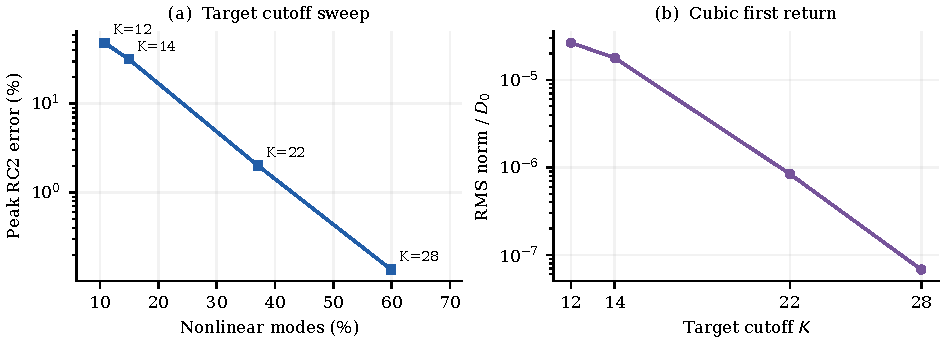
\includegraphics[width=.80\textwidth]{figures/figS1_diagnostics.pdf}
\caption{Additional preparation diagnostics at $\mathrm{Re}=10^5$, $(N_c,N_t)=(32,64)$. (a) Peak RC2 error through $t^*=3$ versus the fraction of modes retained nonlinearly; squares mark the four computed cutoffs, $K=12,14,22,28$. (b) RMS cubic first-return norm defined in Eq.~\eqref{eq:returns}, evaluated along the nonlinear quadratic residual solution. Lines guide the eye; neither diagnostic is the pilot criterion or an error bound.}
\label{fig:diagnostics}
\end{figure}

\clearpage
\begin{table}[h]
\centering\small
\caption{Final errors at $t^*=3$ on $(N_c,N_t)=(32,64)$, $\mathrm{Re}=10^5$. Population errors use the main-text normalization; vorticity errors use the current reference norm. The quadratic solution is evolved without lifting.}
\begin{tabular}{rrrrrr}\toprule
$K$ & Modes & Fraction (\%) & RC2 (\%) & Nonlinear quadratic (\%) & RC2 vorticity (\%)\\\midrule
12 &441 &10.77&48.6331&$9.09\times10^{-3}$&356.415\\
14 &613 &14.97&31.7445&$5.42\times10^{-3}$&222.468\\
22 &1517&37.04&1.8664&$2.93\times10^{-4}$&11.770\\
28 &2453&59.89&0.1358&$2.48\times10^{-5}$&0.904\\\bottomrule
\end{tabular}
\end{table}
The cubic diagnostic decreases from $2.6551\times10^{-5}$ at $K=12$ to $8.4140\times10^{-7}$ at 22 and $6.8025\times10^{-8}$ at 28. The corresponding RC2 errors also decrease strongly. This trend supports the defect mechanism. At the more moderate $\mathrm{Re}=1198.08$, the $K=12$ preparation gives final RC2 errors $0.00243\%$ and $0.00639\%$ for $(N_c,N_t)=(16,32)$ and $(32,64)$, respectively.

\textit{Population checks.} The conventional C2 run uses the same $64^2$ initial state and reference: its final error is $87.343\%$ (peak $102.059\%$). Nonlinear evolution of its fixed-rest quadratic equation gives $0.758\%$ final error. Reference snapshots agree exactly with the RC2 reference. Full nonlinear residual identity checks against direct six-field and independently implemented nine-population LB updates gave maximum normalized differences below $2.2\times10^{-11}$ and $4.1\times10^{-11}$ for the tested $(N_c,N_t)=(16,32),(16,64),(32,64)$ cases, both Reynolds numbers, and $K=8,12$. These are ratios, not percentages. No fine-reference state is substituted during lifted evolution.


\textit{Mode counts and checks.} Counts include the zero mode and count conjugate pairs as two real degrees of freedom; multiplying by six gives the nonlinear dimension. The residual dimension remains $6N_t^2$, with no pair-sector mask. At $K=28$, all prolonged $32^2$ support lies inside the projector, so $c_0=P_{28}f_0$ and $c_{n+1}=P_{28}\F_t(c_n)$, computed on $64^2$ sites. This simplification follows after cutoff selection; eliminating the coarse signal is not the selection criterion. The pilot sweep still uses the transferred coarse trajectory. The implementation evaluates the nonlinear target map before projection; retained-mode counts do not measure runtime savings. Errors are recorded each step in double precision. Vorticity uses Fourier differentiation of $\bm j/\rho$; plotted fields are unsmoothed.

\newpage
\section*{S6. Implementation reference: Fourier transfer and indexed updates}
This section makes the spatial operations and population contractions explicit. Equations in S1--S3 define the same algorithm; no additional closure or approximation is introduced here. The state is sampled after collision, so every LB step streams first and collides second. The main-text construction and its numerical results are unchanged.

\subsection*{S6.1. Discrete Fourier conventions, prolongation, and projection}
Let $\bm\ell=(\ell_x,\ell_y)\in\{0,\ldots,N-1\}^2$ label lattice nodes, with physical coordinates $\bm x=\bm\ell/N$ in the periodic unit square. For the even grids used here, choose the signed frequency set $\mathcal K_N=\{-N/2,\ldots,N/2-1\}$. For each population component, our normalized forward transform and inverse are
\begin{align}
 \widehat h_i^{(N)}(\bm k)&=\frac1{N^2}\sum_{\bm\ell}h_i^{(N)}(\bm\ell)
 \exp[-2\pi\mathrm i\,\bm k\cdot\bm\ell/N],\quad \bm k\in\mathcal K_N^2,\label{eq:dft}\\
 h_i^{(N)}(\bm\ell)&=\sum_{\bm k\in\mathcal K_N^2}\widehat h_i^{(N)}(\bm k)
 \exp[2\pi\mathrm i\,\bm k\cdot\bm\ell/N].\label{eq:idft}
\end{align}
Here $\mathrm i$ is the imaginary unit; $i$ as a subscript labels populations. Fourier wave numbers are integer mode indices; the physical angular wavevector in the unit domain is $2\pi\bm k$. FFT arrays may store these indices in wrapped order without changing either formula. Real fields have conjugate symmetry, with negative frequencies interpreted modulo $N$.

\textit{Spatial prolongation.} For $N_t>N_c$, prolongation evaluates the coarse trigonometric interpolant at target nodes. To specify the even-grid convention unambiguously, define a one-dimensional coefficient embedding
\begin{equation}
 T_{pq}=\begin{cases}
 1,&q\ne-N_c/2,\ p=q,\\
 1/2,&q=-N_c/2,\ p=-N_c/2\ \text{or}\ p=N_c/2,\\
 0,&\text{otherwise},
 \end{cases}
 \quad q\in\mathcal K_{N_c},\ p\in\mathcal K_{N_t}.
\end{equation}
The prolonged normalized coefficients and field are
\begin{align}
 \widehat b_i(p_x,p_y;m)
 &=\sum_{q_x,q_y\in\mathcal K_{N_c}}T_{p_xq_x}T_{p_yq_y}
 \widehat g_i^{(N_c)}(q_x,q_y;m),\label{eq:embed}\\
 (\mathcal P_{c\to t}g_i)(\bm\ell,m)
 &=\sum_{\bm p\in\mathcal K_{N_t}^2}\widehat b_i(\bm p;m)
 \exp[2\pi\mathrm i\,\bm p\cdot\bm\ell/N_t].
\end{align}
Thus a coefficient on one coarse Nyquist line is split equally between its two signed target frequencies; the Nyquist corner is split into four quarters. All other frequencies outside the coarse support are zero. This convention preserves real fields and, for the integer refinement ratios used here, reproduces coarse values at coincident nodes. With an unnormalized forward FFT and an inverse FFT containing $1/N^2$, multiply the embedded coarse FFT coefficients by $(N_t/N_c)^2$ before the target inverse FFT. No such factor is needed with Eqs.~\eqref{eq:dft}--\eqref{eq:idft}.

Time interpolation then uses $s=N_t/N_c$, $m=\lfloor n/s\rfloor$, and $\theta=n/s-m$ as in S2. At $\theta=0$, including the final time, use only the state at $m$; no state beyond the prescribed horizon is required. Prolongation acts on each postcollision population, equivalently each of the six linear moment coordinates, with no stress rescaling.

\textit{Target projection.} Define $\chi_K(\bm k)=1$ if $k_x^2+k_y^2\le K^2$ and zero otherwise. Then
\begin{equation}
 (P_Kh)_i(\bm\ell)=\sum_{\bm k\in\mathcal K_{N_t}^2}\chi_K(\bm k)
 \widehat h_i^{(N_t)}(\bm k)\exp[2\pi\mathrm i\,\bm k\cdot\bm\ell/N_t].
 \label{eq:explicitprojection}
\end{equation}
The complement uses $1-\chi_K$. This is an idempotent disk projection, applied separately to all components; it preserves constants and does not act on the residual or its lifted sectors. Target streaming is a cyclic integer shift $h_i^s(\bm\ell)=h_i(\bm\ell-\bm v_i)$; equivalently $\widehat h_i^s(\bm k)=e^{-2\pi\mathrm i\,\bm k\cdot\bm v_i/N_t}\widehat h_i(\bm k)$.

\newpage
\subsection*{S6.2. Target map and its first and second derivatives}
All node labels in this subsection are target integer indices, and all shifts are modulo $N_t$. For arbitrary input $h$, stream $h_i^s(\bm\ell)=h_i(\bm\ell-\bm v_i)$ and compute $\rho=\sum_i h_i^s$, $j_\alpha=\sum_i v_{i\alpha}h_i^s$. Using the equilibrium and stress projector in S1,
\begin{equation}
 [\F_t(h)]_i(\bm\ell)=f_i^{\rm eq}(\rho,\bm j)
 +(1-\omega_t)[\mathcal R_2(h^s-f^{\rm eq})]_i,
 \qquad \omega_t=1/\tau_{N_t}.
 \label{eq:explicitmap}
\end{equation}
In particular, evaluate $c_i^\star=[\F_t(c_n)]_i$ once, then use
\begin{equation}
 c_{i,n+1}=P_Kc_i^\star+(I-P_K)b_{i,n+1},\qquad
 d_{i,n}=c_i^\star-c_{i,n+1}=(I-P_K)(c_i^\star-b_{i,n+1}).
\end{equation}
This is a nonlinear target-grid evaluation followed by projection. Retained modes follow the target update; complementary background modes follow the transferred coarse trajectory. The defect reuses the trial update, so it needs no second LB evaluation. Although $P_Kd_n=0$, the subsequent residual need not remain in the complementary sector.

To differentiate, stream $c_n$ and form $\rho_c,\bm j_c$, and $\bm u_c=\bm j_c/\rho_c$. For any perturbation $h$, set $\delta\rho_h=\sum_jh_j^s$, $\delta j_{h\alpha}=\sum_jv_{j\alpha}h_j^s$, and $\xi_{h\alpha}=\delta j_{h\alpha}-u_{c\alpha}\delta\rho_h$. All background coefficients below are local to the destination node and step. Define
\begin{align}
 L_{\alpha j}&=v_{j\alpha}-u_{c\alpha},\notag\\
 e_{ij}&=w_i\left[1+\frac{v_{i\alpha}v_{j\alpha}}{c_s^2}
 +\frac{H_{i\alpha\beta}}{2c_s^4}
 (u_{c\alpha}v_{j\beta}+v_{j\alpha}u_{c\beta}-u_{c\alpha}u_{c\beta})\right],\\
 R_{ij}&=\frac{w_iH_{i\alpha\beta}H_{j\alpha\beta}}{2c_s^4},\qquad
 C_{ij}=e_{ij}+(1-\omega_t)\left(R_{ij}-\sum_pR_{ip}e_{pj}\right).
\end{align}
Here $e_{ij}=\partial f_i^{\rm eq}/\partial h_j^s$ and $R_{ij}$ represents $\mathcal R_2$. The full Jacobian action, including streaming, is
\begin{equation}
 (A_nh)_i(\bm\ell)=\sum_jC_{ij}(\bm\ell,n)h_j(\bm\ell-\bm v_j),\qquad
 A_{i\bm\ell,j\bm y}(n)=C_{ij}(\bm\ell,n)\delta^{\rm per}_{\bm y,\bm\ell-\bm v_j}.
 \label{eq:explicitA}
\end{equation}
This is exactly the equilibrium-variation formulation in S2. For two perturbations $h,k$, direct differentiation of the rational equilibrium gives
\begin{equation}
 D^2\!\left(\frac{j_\alpha j_\beta}{\rho}\right)[h,k]
 =\frac{\xi_{h\alpha}\xi_{k\beta}+\xi_{k\alpha}\xi_{h\beta}}{\rho_c}.
\end{equation}
This variation lies in the stress subspace, where $\mathcal R_2$ is the identity; hence differentiating Eq.~\eqref{eq:explicitmap} twice supplies $\omega_t$. With $\B_n=\tfrac12D^2\F_t(c_n)$,
\begin{align}
 [\B_n(h\otimes k)]_i(\bm\ell)
 &=\frac{\omega_t w_iH_{i\alpha\beta}}{4c_s^4\rho_c}
 (\xi_{h\alpha}\xi_{k\beta}+\xi_{k\alpha}\xi_{h\beta})\notag\\
 &=\sum_{j,p}\beta_{i;jp}(\bm\ell,n)
 h_j(\bm\ell-\bm v_j)k_p(\bm\ell-\bm v_p),\qquad
 \beta_{i;jp}=\frac{\omega_t w_iH_{i\alpha\beta}L_{\alpha j}L_{\beta p}}{2c_s^4\rho_c}.
 \label{eq:explicitB}
\end{align}
Symmetry of $H$ makes $\beta_{i;jp}=\beta_{i;pj}$. The exact nonlinear residual replaces $\rho_c$ by $\rho_c+\delta\rho_r$ in the rank-one quadratic expression, giving the exact remainder in S4. These expressions assume nonzero densities; the physical regime has positive background and reconstructed densities.

\newpage
\subsection*{S6.3. Fully indexed RC2 step and execution order}
Write $r_i(\bm\ell,n)$ for the first sector and $Z_{jp}(\bm y,\bm z,n)$ for the independent pair sector. From the local coefficients in Eqs.~\eqref{eq:explicitA}--\eqref{eq:explicitB}, first compute
\begin{align}
 q_i(\bm\ell,n)&=\sum_{j,p}\beta_{i;jp}(\bm\ell,n)
 Z_{jp}(\bm\ell-\bm v_j,\bm\ell-\bm v_p,n),\label{eq:indexedq}\\
 s_i(\bm\ell,n)&=\sum_jC_{ij}(\bm\ell,n)r_j(\bm\ell-\bm v_j,n)+q_i(\bm\ell,n).
\end{align}
The two incoming populations in Eq.~\eqref{eq:indexedq} generally originate at different nodes. The contraction uses these streamed spatial pairs, not products reconstructed from the first sector. Advance
\begin{align}
 r_i(\bm\ell,n+1)&=d_i(\bm\ell,n)+s_i(\bm\ell,n),\label{eq:indexedr}\\
 Z_{ip}(\bm\ell,\bm z,n+1)
 &=\sum_{j,k}C_{ij}(\bm\ell,n)C_{pk}(\bm z,n)
 Z_{jk}(\bm\ell-\bm v_j,\bm z-\bm v_k,n)\notag\\
 &\quad+d_i(\bm\ell,n)s_p(\bm z,n)+s_i(\bm\ell,n)d_p(\bm z,n)
 +d_i(\bm\ell,n)d_p(\bm z,n).
 \label{eq:indexedZ}
\end{align}
Each factor of the pair propagates with its own destination-node coefficients. Every right-hand side uses the old sectors and the prescribed background at step $n$; updates must not overwrite data still needed in that step. Initialize only once:
\begin{equation}
 r_i(\bm\ell,0)=f_i(\bm\ell,0)-c_i(\bm\ell,0),\qquad
 Z_{ip}(\bm\ell,\bm z,0)=r_i(\bm\ell,0)r_p(\bm z,0).
\end{equation}
The output is $f_i^{\rm RC2}(\bm\ell,n)=c_i(\bm\ell,n)+r_i(\bm\ell,n)$. It is never fed back into background preparation. The exact factor representation in S3.2 evaluates these same equations without storing the full pair array.

\textit{Implementation sequence.}
\begin{enumerate}
\item Specify the flow, $T^*$, lattice pair, and relaxation times. On the pilot pair, compute the shared nonlinear trajectories, screen the predefined cutoffs, and transfer the selected $K'/N_t'$ to the target pair as in S5.
\item Compute the independent coarse trajectory through the required horizon and obtain $b_n$ at target times using S6.1. Initialize $c_0=P_Kf_0+(I-P_K)b_0$, $r_0=f_0-c_0$, and its rank-one pair.
\item At target step $n$, stream $c_n$, compute its moments, evaluate the trial update $c^\star$, and obtain $c_{n+1}$ and $d_n$. Form $C$ and $\beta$ from the streamed $c_n$, not from $c_{n+1}$ or from the reconstructed solution.
\item Contract the old pair for $q_n$, form $s_n$, and advance both sectors by Eqs.~\eqref{eq:indexedr}--\eqref{eq:indexedZ}, or use their exact factor implementation. Output $c_{n+1}+r_{n+1}$.
\item Repeat to the prescribed final step without reconstructing $Z_n$ from $r_n$. The nonlinear quadratic and direct-LB comparison runs are optional diagnostics, not inputs to this target lift.
\end{enumerate}
The background may be computed and stored in advance, or streamed forward alongside the lift because it receives no residual feedback. The target collision is evaluated pointwise on the specified target lattice, then projected. No additional de-aliasing rule is inserted; padding or evaluating the nonlinear collision on a different grid would define a different background map. Fourier smoothing concerns the prepared background, not a smoothing of the reported flow fields.

\end{document}
